\section{Danske Bank}

\begin{quote_highlight}
We have a constant focus on improving our advisory services and developing unique digital products. Our goal is to give our customers the best possible advice and provide them with seamless digital solutions. By continuously developing our offerings and introducing new and innovative tools, we aim to create value for all our customers – from making daily payments easy for our private customers to supporting our large, corporate customers in developing their business \cite{danske_bank_our_essence}
\end{quote_highlight}

Danske bank is the largest bank in Denmark \cite[p.~38]{danske_bank_setting_up_in_denmark}, with 2.7 million personal customers, 238,000 small and medium-sized business customers and 1,700 corporate and institutional customers, across the Nordic countries and in Northern Ireland. Danske bank offers a wide range of banking services for Danish and international customers, promising highly available and feature rich digital solutions. Danske bank is active in many sectors within the fields of banking, providing comprehensive digital solutions within each, resulting in several high-end digital solutions. Current solutions include comprehensive web solutions, tablet and smarthphones applications for personal banking and a leading mobile payment application with more than 400.000 transactions daily. Danske bank prioritizes being on the technological forefront, deeming it highly important for customer satisfaction and retainment. 

\subsection*{Notes}
Developing, expanding and maintaining a so comprehensive digital infrastructure is very demanding and complex. 
Being the first Danish bank to release mobile banking and mobile payment on smartphones 
Complex infrastructure
Data handling
1 mill transactions

\subsection{The shared database}

\begin{quote_highlight}
\textbf{The Shared Database:} By far the most common form of integration that I or any of my colleagues see in the industry is database (DB) integration [...] This is really simple when you first think about it, and is probably the faster form of integration to start with [...] but it's one fraught with difficulties \cite[p.~41]{newman2015microservices}
\end{quote_highlight}

Danske bank has a high amount of existing systems, servicing many different areas of the customer segment. Several areas of the existing infrastructure has been identified as 'in need of reiteration', where current demands has outgrown the potential of reliable but rigid older monolithic systems. Earlier developed systems have not been developed with current scale and performance requirements in mind, and are therefore under high pressure, imposing limitations on the organisation as a whole. Current and future redevelopment and expansions of the existing systems have therefore been scheduled and planned. 


A specific challenge has been identified, involving a very limited area of a solution within the Danske bank infrastructure. A overview of the specific challenge is seen on Figure \ref{fig:shared_database}. The existing solution consists of a Admin system, a proxy system and a high amount of diverse consumers. The admin system is responsible for writing and maintaining a database, which is accessed by a proxy making database data available for interested applications. Consumers read database data through the proxy, that ensures the required form of database access control.

\begin{figure}[!htb]
  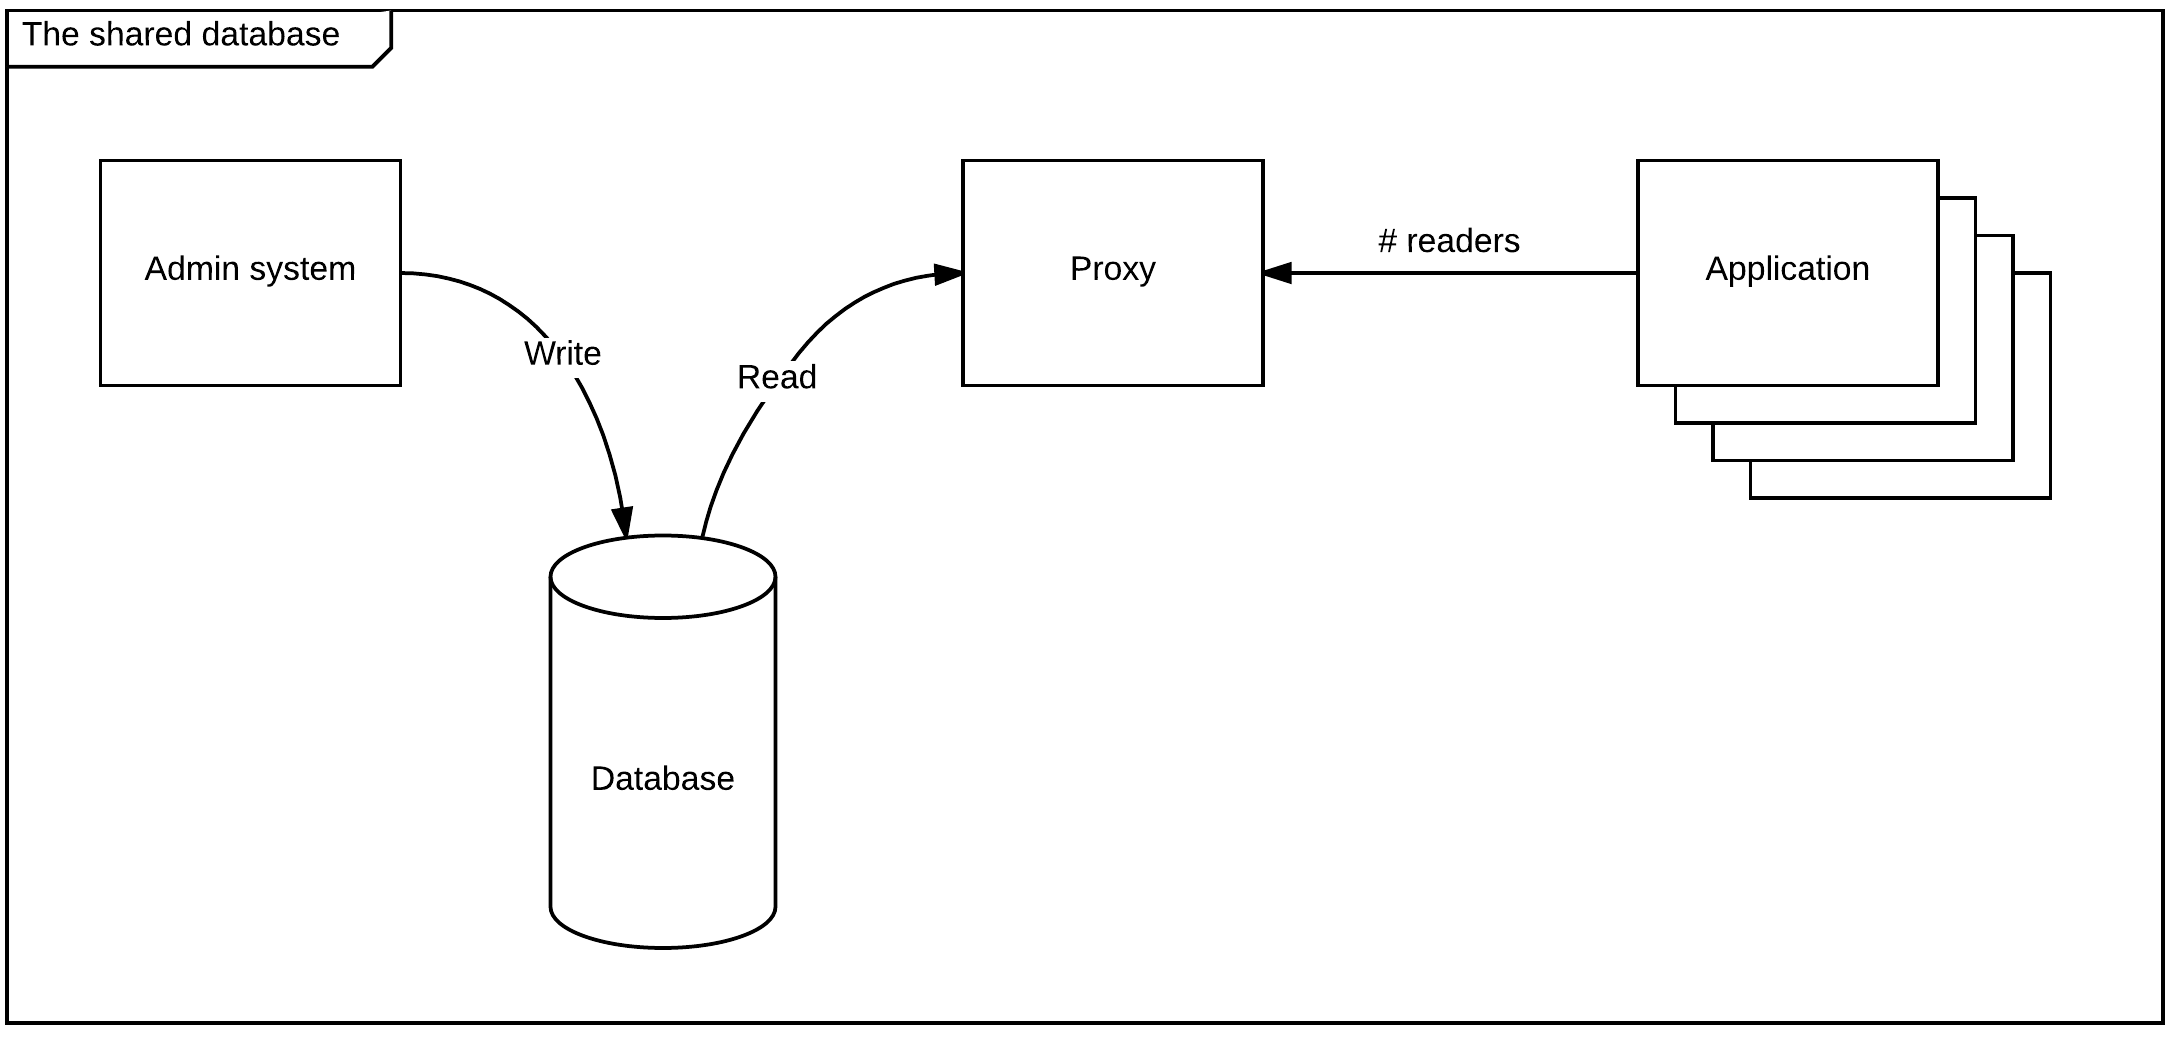
\includegraphics[scale=0.2]{shared_database}  
  \caption{Current solution, with a shared database}
  \label{fig:shared_database}
\end{figure}

\subsection{Challenges with a shared database}
Danske bank has identified a number of challenges with the current implementation. 

\comment{All following sections should be expanded}
\subsubsection{Limited scalability}
The access control Proxy together with the current database implementation is effectively acting as a bottleneck within the system, setting the ceiling for achievable system throughput.

\subsubsection{Single point of failure}
Each consumer is highly reliant on a correct and running administrator system and database. All clients are communicating with the same proxy and database, inferring a very high responsibility on each consumer, a incorrect implementation could cause the proxy or database to collapse, due to malformed or a high amount of requests from a single or several consumers.

\subsubsection{High coupling}
Each client is implemented according to the current proxy and database technology choice, changing either would infer changes in all consumers.
\comment{I am not totally sure we can say this? Depends on whether my understanding of the proxy is correct?} 
This coupling goes both ways, where requirements for a very high read access rate, limits usable database implementation choices.

\subsubsection{Loss of cohesion}
Interpretation of the database is done within each consumer, inferring potential duplication of consumer implementation.
\comment{I am not totally sure we can say this? Depends on whether my understanding of the proxy is correct?} 


\subsection{Where Danske bank want to go}
Distribute responsibility, each consumer wanting to subscribe to the data source, has it's own representation of the data, moving responsibility from the single database to a consumer database. Adding more consumers does hereby not introduce risk on all other consumers, by burdening a central database.


A more scalable solution, where an unlimited number of consumers can be added, solving limitations in the current implementation. Not limiting database implementation, making it possible to swap individual parts of the system without incurring change on the rest of the system.

\comment{Add more reasons.}

\subsection*{Notes}
\say{The Group offers Danish and international customers a wide range of services in the fields of banking, mortgage finance, insurance, leasing, real-estate brokerage and asset management} 


Danske bank has been in constant development, modernizing existing and creating new systems, with a focus on 
focusing on creating highly available, consistent and scalable solutions.


No JOINS on table, too slow


Properly not a very good Normalization form


In need of something that can server a lot of reads


External parties view and bind internal implementation

Logic associated with interpreting and changing data is spread out, if some logic contains a bug or the database is changed, it infers changes multiple places, removing cohesion